\documentclass[tikz,border=7pt]{standalone}
\usepackage{amsmath,pgfplots}
\pgfplotsset{compat=1.18}
\begin{document}
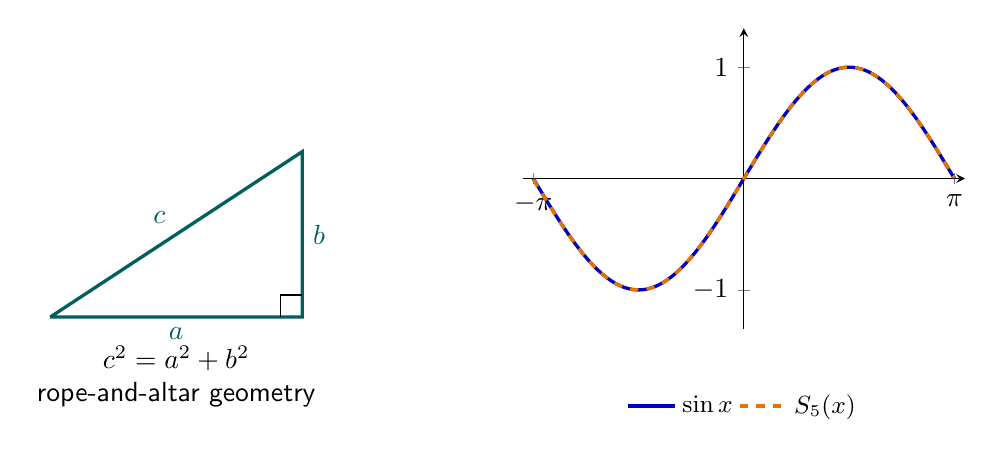
\begin{tikzpicture}[font=\sffamily]
\begin{scope}
\coordinate (A) at (0,0);\coordinate (B) at (3.2,0);\coordinate (C) at (3.2,2.1);
\draw[very thick,teal!75!black] (A)--node[below]{$a$}(B)--node[right]{$b$}(C)--node[above left]{$c$}(A);
\draw (B)+(-.28,0)--+(-.28,.28)--+(0,.28);
\node[align=center] at (1.6,-.75) {$c^2=a^2+b^2$\\rope-and-altar geometry};
\end{scope}
\begin{axis}[at={(6.0cm,-.15cm)},anchor=south west,width=7.2cm,height=5.4cm,
axis lines=middle,xmin=-3.3,xmax=3.3,ymin=-1.35,ymax=1.35,
xtick={-3.1416,0,3.1416},xticklabels={$-\pi$,0,$\pi$},ytick={-1,0,1},
legend style={draw=none,font=\small,at={(.5,-.18)},anchor=north,legend columns=2}]
\addplot[blue!75!black,very thick,domain=-3.1416:3.1416,samples=180]{sin(deg(x))};
\addplot[orange!90!black,dashed,very thick,domain=-3.1416:3.1416,samples=180]{x-x^3/6+x^5/120-x^7/5040+x^9/362880};
\legend{$\sin x$,$S_5(x)$}
\end{axis}
\end{tikzpicture}
\end{document}
